\documentclass{report}

%%%%%%%%%%%%%%%%%%%%%%%%%%%%%%%%%
% PACKAGE IMPORTS
%%%%%%%%%%%%%%%%%%%%%%%%%%%%%%%%%

\usepackage[utf8]{inputenc} % Сурс - семинары по алгебре Медведя Никиты Юрьевича
\usepackage[T2A]{fontenc}

\usepackage[tmargin=2cm,rmargin=1in,lmargin=1in,margin=0.85in,bmargin=2cm,footskip=.2in]{geometry}
\usepackage{amsmath,amsfonts,amsthm,amssymb,mathtools}
\usepackage[varbb]{newpxmath}
\usepackage{xfrac}
\usepackage[makeroom]{cancel}
\usepackage{mathtools}
\usepackage{bookmark}
\usepackage{enumitem}
\usepackage{hyperref,theoremref}
\hypersetup{
	pdftitle={Assignment},
	colorlinks=true, linkcolor=doc!90,
	bookmarksnumbered=true,
	bookmarksopen=true
}
\usepackage[most,many,breakable]{tcolorbox}
\usepackage{xcolor}% http://ctan.org/pkg/xcolor
%\usepackage{colortbl}% http://ctan.org/pkg/colortbl
\usepackage{multirow}% http://ctan.org/pkg/multirow
\usepackage{graphicx}% http://ctan.org/pkg/graphicx
\usepackage{varwidth}
\usepackage{varwidth}
\usepackage{etoolbox}
\usepackage{anyfontsize}
% \usepackage{lmodern}
%\usepackage{authblk}
\usepackage{nameref}
\usepackage{multicol,array}
\usepackage{tikz-cd}
\usepackage[ruled,vlined,linesnumbered]{algorithm2e}
\usepackage{comment} % enables the use of multi-line comments (\ifx \fi) 
\usepackage{import}
\usepackage{xifthen}
\usepackage{pdfpages}
\usepackage{transparent}

\usepackage[english]{babel}
% ,russian
\usepackage{amsfonts,amssymb}
\usepackage{relsize}

\usepackage{systeme}

\usepackage{indentfirst} % Красная строка
\usepackage{fancyhdr}
\usepackage{wrapfig}
\usepackage{textcomp}

\usepackage{physics}

% \usepackage[unicode]{hyperref}

\newcommand\mycommfont[1]{\footnotesize\ttfamily\textcolor{blue}{#1}}
\SetCommentSty{mycommfont}
\newcommand{\incfig}[1]{%
    \def\svgwidth{\columnwidth}
    \import{./figures/}{#1.pdf_tex}
}

\usepackage{tikzsymbols}
\renewcommand\qedsymbol{$\blacksquare$}

\usepackage{sectsty}

% strikethrough text \sout
\usepackage[normalem]{ulem}

\usepackage{code}

\chapternumberfont{\normalsize} 
\chaptertitlefont{\Large}
% \fontsize{<size>}{<line space>}
\sectionfont{\fontsize{12}{15}\selectfont}

% <chapter>.<section> -> <section> indexing in report mode
% \renewcommand{\thesection}{\arabic{section}}

%\usepackage{import}
%\usepackage{xifthen}
%\usepackage{pdfpages}
%\usepackage{transparent}


%%%%%%%%%%%%%%%%%%%%%%%%%%%%%%
% SELF MADE COLORS
%%%%%%%%%%%%%%%%%%%%%%%%%%%%%%



\definecolor{myg}{RGB}{56, 140, 70}
\definecolor{myb}{RGB}{45, 111, 177}
\definecolor{myr}{RGB}{199, 68, 64}
\definecolor{mytheorembg}{HTML}{F2F2F9}
\definecolor{mytheoremfr}{HTML}{00007B}
\definecolor{mylemmabg}{HTML}{FFFAF8}
\definecolor{mylemmafr}{HTML}{983b0f}
\definecolor{mypropbg}{HTML}{f2fbfc}
\definecolor{mypropfr}{HTML}{191971}
\definecolor{myexamplebg}{HTML}{F2FBF8}
\definecolor{myexamplefr}{HTML}{88D6D1}
\definecolor{myexampleti}{HTML}{2A7F7F}
\definecolor{mydefinitbg}{HTML}{E5E5FF}
\definecolor{mydefinitfr}{HTML}{3F3FA3}
\definecolor{notesgreen}{RGB}{0,162,0}
\definecolor{myp}{RGB}{197, 92, 212}
\definecolor{mygr}{HTML}{2C3338}
\definecolor{myred}{RGB}{127,0,0}
\definecolor{myyellow}{RGB}{169,121,69}
\definecolor{myexercisebg}{HTML}{F2FBF8}
\definecolor{myexercisefg}{HTML}{88D6D1}

\definecolor{myclarificationbg}{HTML}{FFFAF8}
\definecolor{myclarificationfr}{HTML}{983b0f}


%%%%%%%%%%%%%%%%%%%%%%%%%%%%
% TCOLORBOX SETUPS
%%%%%%%%%%%%%%%%%%%%%%%%%%%%

\setlength{\parindent}{1cm}
%================================
% THEOREM BOX
%================================

\tcbuselibrary{theorems,skins,hooks}
\newtcbtheorem[number within=section]{Theorem}{Theorem}
{%
	enhanced,
	breakable,
	colback = mytheorembg,
	frame hidden,
	boxrule = 0sp,
	borderline west = {2pt}{0pt}{mytheoremfr},
	sharp corners,
	detach title,
	before upper = \tcbtitle\par\smallskip,
	coltitle = mytheoremfr,
	fonttitle = \bfseries\sffamily,
	description font = \mdseries,
	separator sign none,
	segmentation style={solid, mytheoremfr},
}
{th}

\tcbuselibrary{theorems,skins,hooks}
\newtcbtheorem[number within=chapter]{theorem}{Theorem}
{%
	enhanced,
	% breakable,
	colback = mytheorembg,
	frame hidden,
	boxrule = 0sp,
	borderline west = {2pt}{0pt}{mytheoremfr},
	sharp corners,
	detach title,
	before upper = \tcbtitle\par\smallskip,
	coltitle = mytheoremfr,
	fonttitle = \bfseries\sffamily,
	description font = \mdseries,
	separator sign none,
	segmentation style={solid, mytheoremfr},
}
{th}


\tcbuselibrary{theorems,skins,hooks}
\newtcolorbox{Theoremcon}
{%
	enhanced
	,breakable
	,colback = mytheorembg
	,frame hidden
	,boxrule = 0sp
	,borderline west = {2pt}{0pt}{mytheoremfr}
	,sharp corners
	,description font = \mdseries
	,separator sign none
}

%================================
% Corollery
%================================
\tcbuselibrary{theorems,skins,hooks}
\newtcbtheorem[number within=section]{Corollary}{Corollary}
{%
	enhanced
	,breakable
	,colback = myp!10
	,frame hidden
	,boxrule = 0sp
	,borderline west = {2pt}{0pt}{myp!85!black}
	,sharp corners
	,detach title
	,before upper = \tcbtitle\par\smallskip
	,coltitle = myp!85!black
	,fonttitle = \bfseries\sffamily
	,description font = \mdseries
	,separator sign none
	,segmentation style={solid, myp!85!black}
}
{th}
\tcbuselibrary{theorems,skins,hooks}
\newtcbtheorem[number within=chapter]{corollary}{Corollary}
{%
	enhanced,
	% breakable,
	colback = myp!10,
	frame hidden,
	boxrule = 0sp,
	borderline west = {2pt}{0pt}{myp!85!black},
	sharp corners,
	detach title,
	before upper = \tcbtitle\par\smallskip,
	coltitle = myp!85!black,
	fonttitle = \bfseries\sffamily,
	description font = \mdseries,
	separator sign none,
	segmentation style={solid, myp!85!black}
}
{th}


%================================
% LENMA
%================================

\tcbuselibrary{theorems,skins,hooks}
\newtcbtheorem[number within=section]{Lemma}{Lemma}
{%
	enhanced,
	breakable,
	colback = mylemmabg,
	frame hidden,
	boxrule = 0sp,
	borderline west = {2pt}{0pt}{mylemmafr},
	sharp corners,
	detach title,
	before upper = \tcbtitle\par\smallskip,
	coltitle = mylemmafr,
	fonttitle = \bfseries\sffamily,
	description font = \mdseries,
	separator sign none,
	segmentation style={solid, mylemmafr},
}
{th}

\tcbuselibrary{theorems,skins,hooks}
\newtcbtheorem[number within=chapter]{lemma}{Lemma}
{%
	enhanced,
	% breakable,
	colback = mylemmabg,
	frame hidden,
	boxrule = 0sp,
	borderline west = {2pt}{0pt}{mylemmafr},
	sharp corners,
	detach title,
	before upper = \tcbtitle\par\smallskip,
	coltitle = mylemmafr,
	fonttitle = \bfseries\sffamily,
	description font = \mdseries,
	separator sign none,
	segmentation style={solid, mylemmafr},
}
{th}


%================================
% PROPOSITION
%================================

\tcbuselibrary{theorems,skins,hooks}
\newtcbtheorem[number within=section]{Prop}{Proposition}
{%
	enhanced,
	breakable,
	colback = mypropbg,
	frame hidden,
	boxrule = 0sp,
	borderline west = {2pt}{0pt}{mypropfr},
	sharp corners,
	detach title,
	before upper = \tcbtitle\par\smallskip,
	coltitle = mypropfr,
	fonttitle = \bfseries\sffamily,
	description font = \mdseries,
	separator sign none,
	segmentation style={solid, mypropfr},
}
{th}

\tcbuselibrary{theorems,skins,hooks}
\newtcbtheorem[number within=chapter]{prop}{Proposition}
{%
	enhanced,
	% breakable,
	colback = mypropbg,
	frame hidden,
	boxrule = 0sp,
	borderline west = {2pt}{0pt}{mypropfr},
	sharp corners,
	detach title,
	before upper = \tcbtitle\par\smallskip,
	coltitle = mypropfr,
	fonttitle = \bfseries\sffamily,
	description font = \mdseries,
	separator sign none,
	segmentation style={solid, mypropfr},
}
{th}


%================================
% CLAIM
%================================

\tcbuselibrary{theorems,skins,hooks}
\newtcbtheorem[number within=section]{Claim}{Claim}
{%
	enhanced,
	breakable,
	colback = myg!10,
	frame hidden,
	boxrule = 0sp,
	borderline west = {2pt}{0pt}{myg},
	sharp corners,
	detach title,
	before upper = \tcbtitle\par\smallskip,
	coltitle = myg!85!black,
	fonttitle = \bfseries\sffamily,
	description font = \mdseries,
	separator sign none,
	segmentation style={solid, myg!85!black}
}
{th}

\tcbuselibrary{theorems,skins,hooks}
\newtcbtheorem[number within=section]{claim}{Claim}
{%
	enhanced,
	% breakable,
	colback = myg!10,
	frame hidden,
	boxrule = 0sp,
	borderline west = {2pt}{0pt}{myg},
	sharp corners,
	detach title,
	before upper = \tcbtitle\par\smallskip,
	coltitle = myg!85!black,
	fonttitle = \bfseries\sffamily,
	description font = \mdseries,
	separator sign none,
	segmentation style={solid, myg!85!black}
}
{th}


%================================
% Exercise
%================================

\tcbuselibrary{theorems,skins,hooks}
\newtcbtheorem[number within=section]{Exercise}{Exercise}
{%
	enhanced,
	breakable,
	colback = myexercisebg,
	frame hidden,
	boxrule = 0sp,
	borderline west = {2pt}{0pt}{myexercisefg},
	sharp corners,
	detach title,
	before upper = \tcbtitle\par\smallskip,
	coltitle = myexercisefg,
	fonttitle = \bfseries\sffamily,
	description font = \mdseries,
	separator sign none,
	segmentation style={solid, myexercisefg},
}
{th}

\tcbuselibrary{theorems,skins,hooks}
\newtcbtheorem[number within=chapter]{exercise}{Exercise}
{%
	enhanced,
	% breakable,
	colback = myexercisebg,
	frame hidden,
	boxrule = 0sp,
	borderline west = {2pt}{0pt}{myexercisefg},
	sharp corners,
	detach title,
	before upper = \tcbtitle\par\smallskip,
	coltitle = myexercisefg,
	fonttitle = \bfseries\sffamily,
	description font = \mdseries,
	separator sign none,
	segmentation style={solid, myexercisefg},
}
{th}

%================================
% EXAMPLE BOX
%================================

\newtcbtheorem[number within=section]{Example}{Example}
{%
	colback = myexamplebg,
	breakable,
	colframe = myexamplefr,
	coltitle = myexampleti,
	boxrule = 1pt,
	sharp corners,
	detach title,
	before upper=\tcbtitle\par\smallskip,
	fonttitle = \bfseries,
	description font = \mdseries,
	separator sign none,
	description delimiters parenthesis
}
{ex}

\newtcbtheorem[number within=chapter]{example}{Example}
{%
	colback = myexamplebg,
	% breakable,
	colframe = myexamplefr,
	coltitle = myexampleti,
	boxrule = 1pt,
	sharp corners,
	detach title,
	before upper=\tcbtitle\par\smallskip,
	fonttitle = \bfseries,
	description font = \mdseries,
	separator sign none,
	description delimiters parenthesis
}
{ex}

%================================
% DEFINITION BOX
%================================

\newtcbtheorem[number within=section]{Definition}{Definition}{enhanced,
	before skip=2mm,after skip=2mm, colback=red!5,colframe=red!80!black,boxrule=0.5mm,
	attach boxed title to top left={xshift=1cm,yshift*=1mm-\tcboxedtitleheight}, varwidth boxed title*=-3cm,
	boxed title style={frame code={
					\path[fill=tcbcolback]
					([yshift=-1mm,xshift=-1mm]frame.north west)
					arc[start angle=0,end angle=180,radius=1mm]
					([yshift=-1mm,xshift=1mm]frame.north east)
					arc[start angle=180,end angle=0,radius=1mm];
					\path[left color=tcbcolback!60!black,right color=tcbcolback!60!black,
						middle color=tcbcolback!80!black]
					([xshift=-2mm]frame.north west) -- ([xshift=2mm]frame.north east)
					[rounded corners=1mm]-- ([xshift=1mm,yshift=-1mm]frame.north east)
					-- (frame.south east) -- (frame.south west)
					-- ([xshift=-1mm,yshift=-1mm]frame.north west)
					[sharp corners]-- cycle;
				},interior engine=empty,
		},
	fonttitle=\bfseries,
	title={#2},#1}{def}
\newtcbtheorem[number within=chapter]{definition}{Definition}{enhanced,
	before skip=2mm,after skip=2mm, colback=red!5,colframe=red!80!black,boxrule=0.5mm,
	attach boxed title to top left={xshift=1cm,yshift*=1mm-\tcboxedtitleheight}, varwidth boxed title*=-3cm,
	boxed title style={frame code={
					\path[fill=tcbcolback]
					([yshift=-1mm,xshift=-1mm]frame.north west)
					arc[start angle=0,end angle=180,radius=1mm]
					([yshift=-1mm,xshift=1mm]frame.north east)
					arc[start angle=180,end angle=0,radius=1mm];
					\path[left color=tcbcolback!60!black,right color=tcbcolback!60!black,
						middle color=tcbcolback!80!black]
					([xshift=-2mm]frame.north west) -- ([xshift=2mm]frame.north east)
					[rounded corners=1mm]-- ([xshift=1mm,yshift=-1mm]frame.north east)
					-- (frame.south east) -- (frame.south west)
					-- ([xshift=-1mm,yshift=-1mm]frame.north west)
					[sharp corners]-- cycle;
				},interior engine=empty,
		},
	fonttitle=\bfseries,
	title={#2},#1}{def}



%================================
% Solution BOX
%================================

\makeatletter
\newtcolorbox{solution}{enhanced,
	breakable,
	colback=white,
	colframe=myg!80!black,
	attach boxed title to top left={yshift*=-\tcboxedtitleheight},
	title=Solution,
	boxed title size=title,
	boxed title style={%
			sharp corners,
			rounded corners=northwest,
			colback=tcbcolframe,
			boxrule=0pt,
		},
	underlay boxed title={%
			\path[fill=tcbcolframe] (title.south west)--(title.south east)
			to[out=0, in=180] ([xshift=5mm]title.east)--
			(title.center-|frame.east)
			[rounded corners=\kvtcb@arc] |-
			(frame.north) -| cycle;
		},
}
\makeatother

%================================
% Question BOX
%================================

\makeatletter
\newtcbtheorem{Question}{Question}{enhanced,
	breakable,
	colback=white,
	colframe=mygr,
	attach boxed title to top left={yshift*=-\tcboxedtitleheight},
	fonttitle=\bfseries,
	title={#2},
	boxed title size=title,
	boxed title style={%
			sharp corners,
			rounded corners=northwest,
			colback=tcbcolframe,
			boxrule=0pt,
		},
	underlay boxed title={%
			\path[fill=tcbcolframe] (title.south west)--(title.south east)
			to[out=0, in=180] ([xshift=5mm]title.east)--
			(title.center-|frame.east)
			[rounded corners=\kvtcb@arc] |-
			(frame.north) -| cycle;
		},
	#1
}{def}
\makeatother

\makeatletter
\newtcbtheorem{question}{Question}{enhanced,
	% breakable,
	colback=white,
	colframe=mygr,
	attach boxed title to top left={yshift*=-\tcboxedtitleheight},
	fonttitle=\bfseries,
	title={#2},
	boxed title size=title,
	boxed title style={%
			sharp corners,
			rounded corners=northwest,
			colback=tcbcolframe,
			boxrule=0pt,
		},
	underlay boxed title={%
			\path[fill=tcbcolframe] (title.south west)--(title.south east)
			to[out=0, in=180] ([xshift=5mm]title.east)--
			(title.center-|frame.east)
			[rounded corners=\kvtcb@arc] |-
			(frame.north) -| cycle;
		},
	#1
}{def}
\makeatother

\newtcbtheorem[number within=chapter]{wconc}{Wrong Concept}{
	breakable,
	enhanced,
	colback=white,
	colframe=myr,
	arc=0pt,
	outer arc=0pt,
	fonttitle=\bfseries\sffamily\large,
	colbacktitle=myr,
	attach boxed title to top left={},
	boxed title style={
			enhanced,
			skin=enhancedfirst jigsaw,
			arc=3pt,
			bottom=0pt,
			interior style={fill=myr}
		},
	#1
}{def}



%================================
% NOTE BOX
%================================

\usetikzlibrary{arrows,calc,shadows.blur}
\tcbuselibrary{skins}
\newtcolorbox{note}[1][]{%
	enhanced jigsaw,
	colback=gray!20!white,%
	colframe=gray!80!black,
	size=small,
	boxrule=1pt,
	title=\textbf{Note},
	halign title=flush center,
	coltitle=black,
	breakable,
	drop shadow=black!50!white,
	attach boxed title to top left={xshift=1cm,yshift=-\tcboxedtitleheight/2,yshifttext=-\tcboxedtitleheight/2},
	minipage boxed title=1.5cm,
	boxed title style={%
			colback=white,
			size=fbox,
			boxrule=1pt,
			boxsep=2pt,
			underlay={%
					\coordinate (dotA) at ($(interior.west) + (-0.5pt,0)$);
					\coordinate (dotB) at ($(interior.east) + (0.5pt,0)$);
					\begin{scope}
						\clip (interior.north west) rectangle ([xshift=3ex]interior.east);
						\filldraw [white, blur shadow={shadow opacity=60, shadow yshift=-.75ex}, rounded corners=2pt] (interior.north west) rectangle (interior.south east);
					\end{scope}
					\begin{scope}[gray!80!black]
						\fill (dotA) circle (2pt);
						\fill (dotB) circle (2pt);
					\end{scope}
				},
		},
	#1,
}

%================================
% Clarification box
%================================

\newtcbtheorem[number within=section]{Clarification}{Clarification}
{%
	colback = myclarificationbg,
	breakable,
	colframe = myclarificationfr,
	coltitle = myexampleti,
	boxrule = 1pt,
	sharp corners,
	detach title,
	before upper=\tcbtitle\par\smallskip,
	fonttitle = \bfseries,
	description font = \mdseries,
	separator sign none,
	description delimiters parenthesis
}
{clarif}

\newtcbtheorem[number within=chapter]{clarification}{Clarification}
{%
	colback = myclarificationbg,
	% breakable,
	colframe = myclarificationfr,
	coltitle = myexampleti,
	boxrule = 1pt,
	sharp corners,
	detach title,
	before upper=\tcbtitle\par\smallskip,
	fonttitle = \bfseries,
	description font = \mdseries,
	separator sign none,
	description delimiters
}
{clarif}

%%%%%%%%%%%%%%%%%%%%%%%%%%%%%%
% SELF MADE COMMANDS
%%%%%%%%%%%%%%%%%%%%%%%%%%%%%%

\newcommand{\nt}[1]{\begin{note}#1\end{note}}

\newcommand{\mcthmBreakable}[2]{\begin{Theorem*}{#1}{}#2\end{Theorem*}}
\newcommand{\mcthm}[2]{\begin{theorem*}{#1}{}#2\end{theorem*}}
\newcommand{\mccorollarBreakable}[2]{\begin{Corollary*}{#1}{}#2\end{Corollary*}}
\newcommand{\mccorollar}[2]{\begin{corollary*}{#1}{}#2\end{corollary*}}
\newcommand{\mcpropBreakable}[2]{\begin{Prop*}{#1}{}#2\end{Prop*}}
\newcommand{\mcprop}[2]{\begin{prop*}{#1}{}#2\end{prop*}}
\newcommand{\mcdfnBreakable}[2]{\begin{Definition*}[colbacktitle=red!75!black]{#1}{}#2\end{Definition*}}
\newcommand{\mcdfn}[2]{\begin{definition*}[colbacktitle=red!75!black]{#1}{}#2\end{definition*}}
\newcommand{\mcexBreakable}[2]{\begin{Example*}{#1}{}#2\end{Example*}}
\newcommand{\mcex}[2]{\begin{example*}{#1}{}#2\end{example*}}
\newcommand{\mcprf}[1]{\begin{mcproof}\[#1\]\end{mcproof}}
\newcommand{\mcproofpure}[1]{\begin{mcproof}#1\end{mcproof}}
\newcommand{\mcclmBreakable}[3]{\begin{Claim*}{#1}{#2}#3\end{Claim*}}
\newcommand{\mcclm}[3]{\begin{claim*}{#1}{#2}#3\end{claim*}}
\newcommand{\mcclarfBreakable}[2]{\begin{Clarification*}{#1}{}#2\end{Clarification*}}
\newcommand{\mcclarf}[2]{\begin{clarification*}{#1}{}#2\end{clarification*}}
\newcommand{\mclemmaBreakable}[2]{\begin{Lemma*}{#1}{}#2\end{Lemma*}}
\newcommand{\mclemma}[2]{\begin{lemma*}{#1}{}#2\end{lemma*}}

\newenvironment{myclaim}[1][\claimname]{\proof[\bfseries #1: ]}{}

\newcommand*\circled[1]{\tikz[baseline=(char.base)]{
		\node[shape=circle,draw,inner sep=1pt] (char) {#1};}}
\newcommand\getcurrentref[1]{%
	\ifnumequal{\value{#1}}{0}
	{??}
	{\the\value{#1}}%
}
\newcommand{\getCurrentSectionNumber}{\getcurrentref{section}}
\newenvironment{mcproof}[1][\proofname]{%
	\proof[\bfseries #1: ]%
}{\endproof}


\newcounter{mylabelcounter}

\makeatletter
\newcommand{\setword}[2]{%
	\phantomsection
	#1\def\@currentlabel{\unexpanded{#1}}\label{#2}%
}
\makeatother


\tikzset{
	symbol/.style={
			draw=none,
			every to/.append style={
					edge node={node [sloped, allow upside down, auto=false]{$#1$}}}
		}
}


% deliminators
% \DeclarePairedDelimiter{\abs}{\lvert}{\rvert}  % declared in <physics>
% \DeclarePairedDelimiter{\norm}{\lVert}{\rVert} % declared in <physics>

\DeclarePairedDelimiter{\ceil}{\lceil}{\rceil}
\DeclarePairedDelimiter{\floor}{\lfloor}{\rfloor}
\DeclarePairedDelimiter{\round}{\lfloor}{\rceil}

\newsavebox\diffdbox
\newcommand{\slantedromand}{{\mathpalette\makesl{d}}}
\newcommand{\makesl}[2]{%
\begingroup
\sbox{\diffdbox}{$\mathsurround=0pt#1\mathrm{#2}$}%
\pdfsave
\pdfsetmatrix{1 0 0.2 1}%
\rlap{\usebox{\diffdbox}}%
\pdfrestore
\hskip\wd\diffdbox
\endgroup
}
\newcommand{\mcdd}[1][]{\ensuremath{\mathop{}\!\ifstrempty{#1}{%
\slantedromand\@ifnextchar^{\hspace{0.2ex}}{\hspace{0.1ex}}}%
{\slantedromand\hspace{0.2ex}^{#1}}}}
\ProvideDocumentCommand\dv{o m g}{%
  \ensuremath{%
    \IfValueTF{#3}{%
      \IfNoValueTF{#1}{%
        \frac{\mcdd #2}{\mcdd #3}%
      }{%
        \frac{\mcdd^{#1} #2}{\mcdd #3^{#1}}%
      }%
    }{%
      \IfNoValueTF{#1}{%
        \frac{\mcdd}{\mcdd #2}%
      }{%
        \frac{\mcdd^{#1}}{\mcdd #2^{#1}}%
      }%
    }%
  }%
}
\providecommand*{\pdv}[3][]{\frac{\partial^{#1}#2}{\partial#3^{#1}}}

% Since the amsthm package isn't loaded

% I prefer the slanted \leq
\let\oldleq\leq % save them in case they're every wanted
\let\oldgeq\geq
\renewcommand{\leq}{\leqslant}
\renewcommand{\geq}{\geqslant}

% % redefine matrix env to allow for alignment, use r as default
% \renewcommand*\env@matrix[1][r]{\hskip -\arraycolsep
%     \let\@ifnextchar\new@ifnextchar
%     \array{*\c@MaxMatrixCols #1}}


%\usepackage{framed}
%\usepackage{titletoc}
%\usepackage{etoolbox}
%\usepackage{lmodern}


%\patchcmd{\tableofcontents}{\contentsname}{\sffamily\contentsname}{}{}

%\renewenvironment{leftbar}
%{\def\FrameCommand{\hspace{6em}%
%		{\color{myyellow}\vrule width 2pt depth 6pt}\hspace{1em}}%
%	\MakeFramed{\parshape 1 0cm \dimexpr\textwidth-6em\relax\FrameRestore}\vskip2pt%
%}
%{\endMakeFramed}

%\titlecontents{chapter}
%[0em]{\vspace*{2\baselineskip}}
%{\parbox{4.5em}{%
%		\hfill\Huge\sffamily\bfseries\color{myred}\thecontentspage}%
%	\vspace*{-2.3\baselineskip}\leftbar\textsc{\small\chaptername~\thecontentslabel}\\\sffamily}
%{}{\endleftbar}
%\titlecontents{section}
%[8.4em]
%{\sffamily\contentslabel{3em}}{}{}
%{\hspace{0.5em}\nobreak\itshape\color{myred}\contentspage}
%\titlecontents{subsection}
%[8.4em]
%{\sffamily\contentslabel{3em}}{}{}  
%{\hspace{0.5em}\nobreak\itshape\color{myred}\contentspage}


%%%%%%%%%%%%%%%%%%%%%%%%%%%%%%%%%%%%%%%%%%%
% TABLE OF CONTENTS
%%%%%%%%%%%%%%%%%%%%%%%%%%%%%%%%%%%%%%%%%%%

\usepackage{tikz}
\definecolor{doc}{RGB}{0,60,110}
\usepackage{titletoc}

% \contentsmargin{0cm}
% \titlecontents{chapter}[3.7pc]
% {\addvspace{30pt}%
% 	\begin{tikzpicture}[remember picture, overlay]%
% 		\draw[fill=doc!60,draw=doc!60] (-7,-.1) rectangle (-0.9,.5);%
% 		\pgftext[left,x=-3.5cm,y=0.2cm]{\color{white}\Large\sc\bfseries Chapter\ \thecontentslabel};%
% 	\end{tikzpicture}\color{doc!60}\large\sc\bfseries}%
% {}
% {}
% {\;\titlerule\;\large\sc\bfseries Page \thecontentspage
% 	\begin{tikzpicture}[remember picture, overlay]
% 		\draw[fill=doc!60,draw=doc!60] (2pt,0) rectangle (4,0.1pt);
% 	\end{tikzpicture}}%
% \titlecontents{section}[3.7pc]
% {\addvspace{2pt}}
% {\contentslabel[\thecontentslabel]{2pc}}
% {}
% {\hfill\small \thecontentspage}
% []
% \titlecontents*{subsection}[3.7pc]
% {\addvspace{-1pt}\small}
% {}
% {}
% {\ --- \small\thecontentspage}
% [ \textbullet\ ][]

% \makeatletter
% \renewcommand{\tableofcontents}{%
% 	\chapter*{%
% 	  \vspace*{-20\p@}%
% 	  \begin{tikzpicture}[remember picture, overlay]%
% 		  \pgftext[right,x=15cm,y=0.2cm]{\color{doc!60}\Huge\sc\bfseries \contentsname};%
% 		  \draw[fill=doc!60,draw=doc!60] (13,-.75) rectangle (20,1);%
% 		  \clip (13,-.75) rectangle (20,1);
% 		  \pgftext[right,x=15cm,y=0.2cm]{\color{white}\Huge\sc\bfseries \contentsname};%
% 	  \end{tikzpicture}}%
% 	\@starttoc{toc}}
% \makeatother


\usepackage{ragged2e}
\usepackage{blindtext}
\usepackage{booktabs}
%From M275 "Topology" at SJSU
\newcommand{\id}{\mathrm{id}}
\newcommand{\taking}[1]{\xrightarrow{#1}}
\newcommand{\inv}{^{-1}}

%From M170 "Introduction to Graph Theory" at SJSU
\DeclareMathOperator{\diam}{diam}
\DeclareMathOperator{\ord}{ord}
\newcommand{\defeq}{\overset{\mathrm{def}}{=}}

%From the USAMO .tex files
\newcommand{\ts}{\textsuperscript}
\newcommand{\dg}{^\circ}
\newcommand{\ii}{\item}

% % From Math 55 and Math 145 at Harvard
% \newenvironment{subproof}[1][Proof]{%
% \begin{proof}[#1] \renewcommand{\qedsymbol}{$\blacksquare$}}%
% {\end{proof}}

\newcommand{\liff}{\leftrightarrow}
\newcommand{\lthen}{\rightarrow}
\newcommand{\opname}{\operatorname}
\newcommand{\surjto}{\twoheadrightarrow}
\newcommand{\injto}{\hookrightarrow}
\newcommand{\On}{\mathrm{On}}        % ordinals
\DeclareMathOperator{\img}{im}       % Image
\DeclareMathOperator{\Img}{Im}       % Image
\DeclareMathOperator{\coker}{coker}  % Cokernel
\DeclareMathOperator{\Coker}{Coker}  % Cokernel
\DeclareMathOperator{\Ker}{Ker}      % Kernel
% \DeclareMathOperator{\rank}{rank}  % rank       % declared in <physics>
\DeclareMathOperator{\Spec}{Spec}    % spectrum
% \DeclareMathOperator{\Tr}{Tr}      % trace      % declared in <physics>
\DeclareMathOperator{\pr}{pr}        % projection
\DeclareMathOperator{\ext}{ext}      % extension
\DeclareMathOperator{\pred}{pred}    % predecessor
\DeclareMathOperator{\dom}{dom}      % domain
\DeclareMathOperator{\ran}{ran}      % range
\DeclareMathOperator{\Hom}{Hom}      % homomorphism
\DeclareMathOperator{\Mor}{Mor}      % morphisms
\DeclareMathOperator{\End}{End}      % endomorphism

\DeclareMathOperator{\lowlim}{\underline{lim}} % lower limit
\DeclareMathOperator{\uplim}{\overline{lim}}   % upper limit

% combinations
\newcommand{\Cmb}[2]{ C^{#2}_{#1} }
\newcommand{\NumSeq}[1]{\{ #1 \}}
\newcommand{\SmO}[1][x]{\overline{o}(#1)}

%probabilities
\newcommand{\Proba}[1]{\mathds{P}\left( #1 \right)}
\newcommand{\Probc}[2]{\mathds{P}\left( #1 ~\vert~ #2\right)}

%expected values
\newcommand{\E}[1]{\mathds{E} \left( #1 \right) }
\newcommand{\Ec}[2]{\mathds{E} \left[ #1 ~\vert ~ #2\right] }

% - others
\DeclareMathOperator{\Lap}{\mathcal{L}}
\DeclareMathOperator{\Var}{var} % varience
\DeclareMathOperator{\cov}{cov} % covarience

\newcommand{\veps}{\varepsilon}
\newcommand{\wt}{\widetilde}
\newcommand{\wh}{\widehat}
\newcommand{\vocab}[1]{\textbf{\color{blue} #1}}
\providecommand{\half}{\frac{1}{2}}
\newcommand{\dang}{\measuredangle} %% Directed angle
\newcommand{\ray}[1]{\overrightarrow{#1}}
\newcommand{\seg}[1]{\overline{#1}}
\newcommand{\arc}[1]{\wideparen{#1}}
\DeclareMathOperator{\cis}{cis}
\DeclareMathOperator*{\lcm}{lcm}

\DeclareMathOperator*{\argmin}{arg min}
\DeclareMathOperator*{\argmax}{arg max}

% Contradiction symbol (like \bot)
\newcommand{\Contradiction}{\ensuremath{\circled{$\mathbb{W}$}}}

\newcommand{\cycsum}{\sum_{\mathrm{cyc}}}
\newcommand{\symsum}{\sum_{\mathrm{sym}}}
\newcommand{\cycprod}{\prod_{\mathrm{cyc}}}
\newcommand{\symprod}{\prod_{\mathrm{sym}}}
\newcommand{\Qed}{\begin{flushright}\qed\end{flushright}}
\newcommand{\parinn}{\setlength{\parindent}{1cm}}
\newcommand{\parinf}{\setlength{\parindent}{0cm}}
% \newcommand{\norm}{\|\cdot\|}                         % declared in <physics>
\newcommand{\inorm}{\norm_{\infty}}
\newcommand{\opensets}{\{V_{\alpha}\}_{\alpha\in I}}
\newcommand{\oset}{V_{\alpha}}
\newcommand{\opset}[1]{V_{\alpha_{#1}}}
\newcommand{\lub}{\text{lub}}
\newcommand{\del}[2]{\frac{\partial #1}{\partial #2}}
\newcommand{\Del}[3]{\frac{\partial^{#1} #2}{\partial^{#1} #3}}
\newcommand{\deld}[2]{\dfrac{\partial #1}{\partial #2}}
\newcommand{\Deld}[3]{\dfrac{\partial^{#1} #2}{\partial^{#1} #3}}
\newcommand{\lm}{\lambda}
\newcommand{\uin}{\mathbin{\rotatebox[origin=c]{90}{$\in$}}}
\newcommand{\usubset}{\mathbin{\rotatebox[origin=c]{90}{$\subset$}}}
\newcommand{\lt}{\left}
\newcommand{\rt}{\right}
\newcommand{\bs}[1]{\boldsymbol{#1}}
\newcommand{\exs}{\exists}
\newcommand{\st}{\strut}
\newcommand{\dps}[1]{\displaystyle{#1}}

\newcommand{\sol}{\setlength{\parindent}{0cm}\textbf{\textit{Solution:}}\setlength{\parindent}{1cm} }
\newcommand{\solve}[1]{\setlength{\parindent}{0cm}\textbf{\textit{Solution: }}\setlength{\parindent}{1cm}#1 \Qed}


\begin{document}

\chapter*{Задание A2}

\section*{Пункт 1.}

\raggedright
В классическом алгоритме Дейкстры на каждом шаге у вершины $v$, до которой сейчас найден ближайший путь, просматриваем
всех соседей $u$ и обновляем расстояния до них как $dist[u] = \min(dist[u], dist[v] + w(v, u))$.

Пользуясь тем, что уже существует доказательство корректности алгоритма Дейкстры, заметим, что в нём используется то,
что веса рёбер неотрицательные и прибавление $w(v, u)$ к $dist[v]$ может уменьшить $dist[u]$, но не сделает его меньше $dist[v]$.

Таким образом, при модификации алгоритма достаточно заменить операцию сложения на умножение и при инициализации расстояние
до стартовой вершины сделать равным 1, а не 0, тогда алгоритм будет работать корректно, если веса всех рёбер неотрицательны.

Если в графе есть ребро $(u, v)$ с отрицательным весом, то до вершины $u$ можно дойти по очень длинному пути, а потом пройти по ребру $(u, v)$,
дойдя до вершины $v$ по пути с большим отрицательным весом
\par

Рассмотрим пример: пусть в ориентированном графе $G = (V, E)$ необходимо найти кратчайший путь из $v_1$ в $v_8$

$\begin{tikzpicture}
    \node[draw,align=left] at (0, 1) {Граф G:};
    \coordinate (v1) at (0, -1);
    \coordinate (v2) at (1, 0);
    \coordinate (v3) at (1, -2);
    \coordinate (v4) at (3, -2);
    \coordinate (v5) at (2, 0);
    \coordinate (v6) at (2.75, -0.5);
    \coordinate (v7) at (3.75, -1);
    \coordinate (v8) at (5.5, -0.25);
    \coordinate (v9) at (2, -3);
    \filldraw[black] (v1) circle (1pt) node[anchor=east]{$v_1$};
    \filldraw[black] (v2) circle (1pt) node[anchor=south]{$v_2$};
    \filldraw[black] (v3) circle (1pt) node[anchor=north]{$v_3$};
    \filldraw[black] (v4) circle (1pt) node[anchor=north west]{$v_4$};
    \filldraw[black] (v5) circle (1pt) node[anchor=south]{$v_5$};
    \filldraw[black] (v6) circle (1pt) node[anchor=south]{$v_6$};
    \filldraw[black] (v7) circle (1pt) node[anchor=south]{$v_7$};
    \filldraw[black] (v8) circle (1pt) node[anchor=west]{$v_8$};
    \filldraw[black] (v9) circle (1pt) node[anchor=north]{$v_9$};
    \draw[-stealth,line width=0.4mm] (v1) -- node[anchor=south]{2} (v2);
    \draw[-stealth,line width=0.4mm] (v1) -- node[anchor=west]{3} (v3);
    \draw[-stealth,line width=0.4mm] (v3) -- node[anchor=north]{7} (v4);
    \draw[-stealth,line width=0.4mm] (v2) -- node[anchor=south]{3} (v5);
    \draw[-stealth,line width=0.4mm] (v2) -- node[anchor=north east]{2} (v4);
    \draw[-stealth,line width=0.4mm] (v5) -- node[anchor=north east]{2} (v6);
    \draw[-stealth,line width=0.4mm] (v6) -- node[anchor=west]{5} (v4);
    \draw[-stealth,line width=0.4mm] (v6) -- node[anchor=south]{2} (v7);
    \draw[-stealth,line width=0.4mm] (v4) -- node[anchor=north]{7} (v8);
    \draw[-stealth,line width=0.4mm] (v5) -- node[anchor=south]{5} (v8);
    \draw[-stealth,line width=0.4mm] (v7) -- node[anchor=south east]{1} (v8);
    \draw[-stealth,line width=0.4mm] (v3) -- node[anchor=north east]{3} (v9);
    \draw[-stealth,line width=0.4mm] (v9) -- node[anchor=north west]{2} (v4);
\end{tikzpicture} $

\begin{align*}
    & \text{Изначально } dist = [ 1, +\infty, +\infty, +\infty, +\infty, +\infty, +\infty, +\infty, +\infty ] \\
    & \text{После посещения } v_1: dist = [ 1, 2, 3, +\infty, +\infty, +\infty, +\infty, +\infty, +\infty, ] \\
    & \text{После посещения } v_2: dist = [ 1, 2, 3, 4, 6, +\infty, +\infty, +\infty, +\infty, ] \\
    & \text{После посещения } v_3: dist = [ 1, 2, 3, 4, 6, +\infty, +\infty, +\infty, 9, ] \\
    & \text{После посещения } v_4: dist = [ 1, 2, 3, 4, 6, +\infty, +\infty, 28, 9, ] \\
    & \text{После посещения } v_5: dist = [ 1, 2, 3, 4, 6, 12, +\infty, 28, 9, ] \\
    & \text{После посещения } v_9: dist = [ 1, 2, 3, 4, 6, 12, +\infty, 28, 9, ] \\
    & \text{После посещения } v_6: dist = [ 1, 2, 3, 4, 6, 12, 24, 28, 9, ] \\
    & \text{После посещения } v_7: dist = [ 1, 2, 3, 4, 6, 12, 24, 24, 9, ] \\
    & \text{После посещения } v_8: dist = [ 1, 2, 3, 4, 6, 12, 24, 24, 9, ] \\
    & \text{Минимальный путь из $v_1$ в $v_8$ - путь } (v_1, v_2, v_5, v_6, v_7, v_8) \text{, вес которого равен 24} \\
\end{align*}

\section*{Пункт 2.}

\raggedright
Пусть, если вершина $v_j$ не достижима из вершины $v_i$ $\implies$ между ними нет кратчайшего пути, то положим $dist[v_i][v_j] = \infty$

1. Сначала для всех пар $1 \le i, j, k \le n$, для которых $ i \ne j \ne k \ne i $ необходимо проверить выполнение неравенства треугольника:

\[
    \left( dist[v_i][v_j] \ne \infty \wedge dist[v_j][v_k] \ne \infty \right)
    \implies
    \left( dist[v_i][v_k] \ne \infty \wedge dist[v_i][v_j] + dist[v_j][v_k] \ge dist[v_i][v_k] \right)
(1) \]

Если оно не выполняется, то приходим к противоречию с определением кратчайшего пути $ \implies $ по такой матрице $dist[][]$
нельзя восстановить граф.

2. При выполнении неравенства рассмотрим такой алгоритм:

В качестве матрицы весов $w$ восстанавливаемого графа положим данную матрицу $dist[][]$ кратчайших путей

А в качестве восстанавливаемого графа $G$ рассмотрим список смежности, построенный из этой матрицы
(вершина $u$ принадлежит списку вершины $v$, если $dist[u][v] \ne inf$)

Это корректно, т.к. если дан ориентированный взвешенный граф $H$, и к нему применили алгоритм Флойда-Уоршелла, получив
матрицу кратчайших путей $dist_H[][]$, то, применив алгоритм Флойда-Уоршелла уже к этой матрице $dist_H[][]$, проинтерпретировав
её как матрицу весов, алгоритм вернёт ту же матрицу $dist_H$ (по факту, ни на одной итерации алгоритма обновление элементов
матрицы не произойдёт, т.к. между вершинами уже найдены оптимальные пути в виду выполнения неравенства треугольника)

В качестве примера рассмотрим матрицу $dist[][]$:

$$
dist = \begin{bmatrix}
     0 & \infty & 4 & \infty & 2 \\
    -1 &  0 & 3 & \infty & 1 \\
     4 & \infty & 0 & \infty & 6 \\
     2 & \infty & 3 &  0 & 4 \\ 
     1 & \infty & 2 & \infty & 0 \\
\end{bmatrix}
$$

Здесь присутствует путь отрицательного веса между вершинами $v_2$ и $v_1$, а также не между любой парой вершин есть путь

Для всех троек элементов данной матриц выполняется неравенство треугольника в форме (1)

Применив к $dist[][]$ алгоритм Флойда-Уоршелла, получим ту же матрицу $dist[][]$

Тогда для восстанавливаемого графа положим матрицу весов равной $ w = dist $ и сформируем список смежности:

\begin{align*}
    L_G = \{ & \\
        v_1: & \, \{ v_3, v_5 \}, \\
        v_2: & \, \{ v_1, v_3, v_5 \}, \\
        v_3: & \, \{ v_1, v_5 \}, \\
        v_4: & \, \{ v_1, v_3, v_5 \} \\
        v_5: & \, \{ v_1, v_3 \} \\
    \} \hspace*{1cm} & \\
\end{align*}

% Для всех пар $ 1 \le i \ne j \le n $, таких что $dist[v_i][v_j] \ne \infty $:

% Если \[ \forall k: k = i \vee k = j \vee dist[v_i][v_k] = \infty \vee dist[v_k][v_j] = \infty \vee dist[v_i][v_k] + dist[v_k][v_j] > dist[v_i][v_j] \]

% то из вершины $v_i$ нельзя попасть в вершину $v_j$ через какую-либо другую вершину.
% Но при этом $dist[v_i][v_j] \ne \infty \implies (v_i, v_j) \in E $,
% т.е. просто соединяем вершины ориентированным ребром

% Иначе, если \[ \exists k: k \ne i \wedge k \ne j \wedge dist[v_i][v_k] \ne \infty \wedge dist[v_k][v_j] \ne \infty \wedge dist[v_i][v_k] + dist[v_k][v_j] = dist[v_i][v_j] \]

% то через такие вершины $v_k$ можно пройти на пути из $v_i$ в $v_j$. Добавим все такие вершины $v_k$ в список вершин, которые могут быть на пути из $v_i$ в $v_j$

\par

\pagebreak

\section*{Пункт 4.}

\raggedright

Т.к. в графе $G = (V, E)$ есть путь  из $a$ в $b$, проходящий через ребро $(v_i, v_j)$, то из вершины
$a$ есть путь $P_{a, v_i}$ до вершины $v_i$ и из вершины $v_j$ есть путь $P_{v_j, b}$ до вершины $b$.
Аналогично, т.к. в графе $G$ есть путь из $b$ в $a$, проходящий через ребро $(v_i, v_j)$, то из вершины 
$b$ есть путь $P_{b, v_i}$ до вершины $v_i$ и из вершины $v_j$ есть путь $P_{v_j, a}$ до вершины $a$.

Следовательно, в графе $G$ есть циклы $P_{a, v_i} \cup \{ (v_i, v_j) \} \cup P_{v_j, a}$ и $P_{b, v_i} \cup \{ (v_i, v_j) \} \cup P_{v_j, b}$.

При этом, кратчайшие пути по условию существуют, то есть из этих циклов не достижимы циклы отрицательного веса, если они есть в графе $G$
(точнее, если и есть ребро из данных циклов в цикл с отрицательным весом, то обратно из этого цикла с отрицательным весом в данные циклы вернуться нельзя),
и сами циклы неотрцательного веса (иначе бы из $a$ в $a$ можно было прийти со сколько угодно малым весом пути)

Пример такого графа:

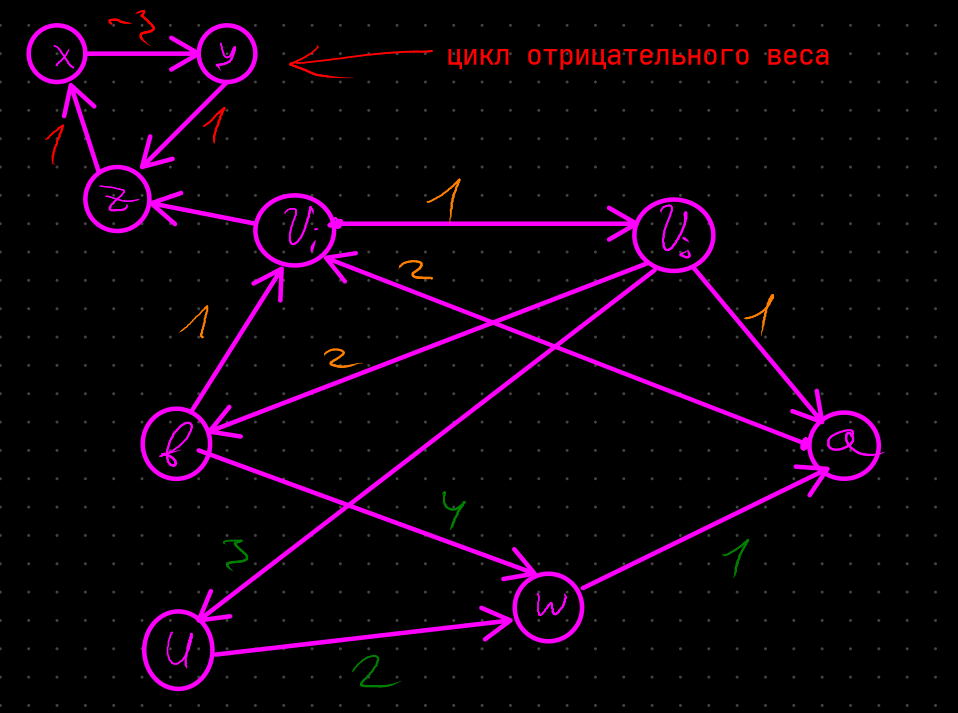
\includegraphics[scale=0.5]{a2_t4.png}

Данные ограничения на граф не гарантируют отсутствие цикла отрицательного веса, но и не накладвают дополнительные ограничения на структуру графа
кроме наличия указанных выше циклов (которые, как показано, неотрицательного веса), а 
алгоритм Дейкстры, A*, Форда-Беллмана и Флойда-Уоршелла корректно работают при наличии циклов, если их вес $\ge 0$.

\par

\pagebreak

\section*{Пункт 3.}

Рассмотрим граф $G = (V, E, w)$, где $ V = \{ 1, 2, 3, 4 \}, E = \{ (1, 2), (2, 3), (3, 4), (4, 1) \} $

Матрица весов графа:
$$
w = \begin{bmatrix}
0 & 1 & +\infty & +\infty \\
+\infty & 0 & 1 & +\infty \\
+\infty & +\infty & 0 & 1 \\
1 & +\infty & +\infty & 0 \\
\end{bmatrix}
$$

$\begin{tikzpicture}
    \node[draw,align=left] at (0, 1) {Граф G:};
    \coordinate (v1) at (0, 0);
    \coordinate (v2) at (2, 0);
    \coordinate (v3) at (2, -2);
    \coordinate (v4) at (0, -2);
    \filldraw[black] (v1) circle (1pt) node[anchor=south]{$v_1$};
    \filldraw[black] (v2) circle (1pt) node[anchor=south]{$v_2$};
    \filldraw[black] (v3) circle (1pt) node[anchor=north]{$v_3$};
    \filldraw[black] (v4) circle (1pt) node[anchor=north]{$v_4$};
    \draw[-stealth] (v1) -- node[anchor=south]{1} (v2);
    \draw[-stealth] (v2) -- node[anchor=west]{1} (v3);
    \draw[-stealth] (v3) -- node[anchor=north]{1} (v4);
    \draw[-stealth] (v4) -- node[anchor=east]{1} (v1);
\end{tikzpicture} $

Инициализация матрицы $dist[][]$
$$
dist = w = \begin{bmatrix}
0 & 1 & +\infty & +\infty \\
+\infty & 0 & 1 & +\infty \\
+\infty & +\infty & 0 & 1 \\
1 & +\infty & +\infty & 0 \\
\end{bmatrix}
$$

\raggedright
Опишем 64 итераций алгоритма в таблице ниже

(латех смещает таблицу в конец документа, вставить её между последующим выводом о получившейся матрице $dist[][]$ и фразой "Опишем 64 итераций..." не получилось)

Получившаяся матрица расстояний:

$\begin{bmatrix}
    0 & 1 & 2 & 3 \\
    +\infty & 0 & 1 & 2 \\
    2 & 3 & 0 & 1 \\
    1 & 2 & 3 & 0 \\
\end{bmatrix}$

Однако корректный алгоритм Флойда-Уоршелла завершает работу, найдя такую матрицу расстояний:

$\begin{bmatrix}
    0 & 1 & 2 & 3 \\
    3 & 0 & 1 & 2 \\
    2 & 3 & 0 & 1 \\
    1 & 2 & 3 & 0 \\
\end{bmatrix}$

Таким образом, некорректный вариант алгоритма не смог найти путь из $v_2$ в $v_1$

\par

\begin{table}[h]
\centering
\begin{tabular}{ccccccc}
\toprule
\multicolumn{1}{c}{} & \multicolumn{3}{c}{\textbf{for cycle values}} & \multicolumn{3}{c}{\textbf{dist values}} \\
\cmidrule(rl){2-4} \cmidrule(rl){5-7}
{$dist[][]$ before update} & {i} & {j} & {k} & {$dist[i][j]$ before update} & {$dist[i][k] + dist[k][j]$} & {$dist[i][j]$ after update} \\
\midrule
$\begin{bmatrix}
    0 & 1 & +\infty & +\infty \\
    +\infty & 0 & 1 & +\infty \\
    +\infty & +\infty & 0 & 1 \\
    1 & +\infty & +\infty & 0 \\
\end{bmatrix}$ & 1 & 1 & 1 & 0 & 0 & 0 \\
\bottomrule
$\begin{bmatrix}
    0 & 1 & +\infty & +\infty \\
    +\infty & 0 & 1 & +\infty \\
    +\infty & +\infty & 0 & 1 \\
    1 & +\infty & +\infty & 0 \\
\end{bmatrix}$ & 1 & 1 & 2 & 0 & $+\infty$ & 0 \\
\bottomrule
$\begin{bmatrix}
    0 & 1 & +\infty & +\infty \\
    +\infty & 0 & 1 & +\infty \\
    +\infty & +\infty & 0 & 1 \\
    1 & +\infty & +\infty & 0 \\
\end{bmatrix}$ & 1 & 1 & 3 & 0 & $+\infty$ & 0 \\
\bottomrule
$\begin{bmatrix}
    0 & 1 & +\infty & +\infty \\
    +\infty & 0 & 1 & +\infty \\
    +\infty & +\infty & 0 & 1 \\
    1 & +\infty & +\infty & 0 \\
\end{bmatrix}$ & 1 & 1 & 4 & 0 & $+\infty$ & 0 \\
\bottomrule
$\begin{bmatrix}
    0 & 1 & +\infty & +\infty \\
    +\infty & 0 & 1 & +\infty \\
    +\infty & +\infty & 0 & 1 \\
    1 & +\infty & +\infty & 0 \\
\end{bmatrix}$ & 1 & 2 & 1 & 1 & 1 & 1 \\
\bottomrule
$\begin{bmatrix}
    0 & 1 & +\infty & +\infty \\
    +\infty & 0 & 1 & +\infty \\
    +\infty & +\infty & 0 & 1 \\
    1 & +\infty & +\infty & 0 \\
\end{bmatrix}$ & 1 & 2 & 2 & 1 & 1 & 1 \\
\bottomrule
$\begin{bmatrix}
    0 & 1 & +\infty & +\infty \\
    +\infty & 0 & 1 & +\infty \\
    +\infty & +\infty & 0 & 1 \\
    1 & +\infty & +\infty & 0 \\
\end{bmatrix}$ & 1 & 2 & 3 & 1 & $+\infty$ & 1 \\
\bottomrule
$\begin{bmatrix}
    0 & 1 & +\infty & +\infty \\
    +\infty & 0 & 1 & +\infty \\
    +\infty & +\infty & 0 & 1 \\
    1 & +\infty & +\infty & 0 \\
\end{bmatrix}$ & 1 & 2 & 4 & 1 & $+\infty$ & 1 \\
\bottomrule
$\begin{bmatrix}
    0 & 1 & +\infty & +\infty \\
    +\infty & 0 & 1 & +\infty \\
    +\infty & +\infty & 0 & 1 \\
    1 & +\infty & +\infty & 0 \\
\end{bmatrix}$ & 1 & 3 & 1 & $+\infty$ & $+\infty$ & $+\infty$ \\
\bottomrule
$\begin{bmatrix}
    0 & 1 & +\infty & +\infty \\
    +\infty & 0 & 1 & +\infty \\
    +\infty & +\infty & 0 & 1 \\
    1 & +\infty & +\infty & 0 \\
\end{bmatrix}$ & 1 & 3 & 2 & $+\infty$ & 2 & 2 \\
\bottomrule
\end{tabular}
\end{table}

\begin{table}[h]
\centering
\begin{tabular}{ccccccc}
\toprule
\multicolumn{1}{c}{} & \multicolumn{3}{c}{\textbf{for cycle values}} & \multicolumn{3}{c}{\textbf{dist values}} \\
\cmidrule(rl){2-4} \cmidrule(rl){5-7}
{$dist[][]$ before update} & {i} & {j} & {k} & {$dist[i][j]$ before update} & {$dist[i][k] + dist[k][j]$} & {$dist[i][j]$ after update} \\
\midrule
$\begin{bmatrix}
    0 & 1 & 2 & +\infty \\
    +\infty & 0 & 1 & +\infty \\
    +\infty & +\infty & 0 & 1 \\
    1 & +\infty & +\infty & 0 \\
\end{bmatrix}$ & 1 & 3 & 3 & 2 & 2 & 2 \\
\bottomrule
$\begin{bmatrix}
    0 & 1 & 2 & +\infty \\
    +\infty & 0 & 1 & +\infty \\
    +\infty & +\infty & 0 & 1 \\
    1 & +\infty & +\infty & 0 \\
\end{bmatrix}$ & 1 & 3 & 4 & 2 & $+\infty$ & 2 \\
\bottomrule
$\begin{bmatrix}
    0 & 1 & 2 & +\infty \\
    +\infty & 0 & 1 & +\infty \\
    +\infty & +\infty & 0 & 1 \\
    1 & +\infty & +\infty & 0 \\
\end{bmatrix}$ & 1 & 4 & 1 & $+\infty$ & $+\infty$ & $+\infty$ \\
\bottomrule
$\begin{bmatrix}
    0 & 1 & 2 & +\infty \\
    +\infty & 0 & 1 & +\infty \\
    +\infty & +\infty & 0 & 1 \\
    1 & +\infty & +\infty & 0 \\
\end{bmatrix}$ & 1 & 4 & 2 & $+\infty$ & $+\infty$ & $+\infty$ \\
\bottomrule
$\begin{bmatrix}
    0 & 1 & 2 & +\infty \\
    +\infty & 0 & 1 & +\infty \\
    +\infty & +\infty & 0 & 1 \\
    1 & +\infty & +\infty & 0 \\
\end{bmatrix}$ & 1 & 4 & 3 & $+\infty$ & 3 & 3 \\
\bottomrule
$\begin{bmatrix}
    0 & 1 & 2 & 3 \\
    +\infty & 0 & 1 & +\infty \\
    +\infty & +\infty & 0 & 1 \\
    1 & +\infty & +\infty & 0 \\
\end{bmatrix}$ & 1 & 4 & 4 & 3 & 3 & 3 \\
\bottomrule
$\begin{bmatrix}
    0 & 1 & 2 & 3 \\
    +\infty & 0 & 1 & +\infty \\
    +\infty & +\infty & 0 & 1 \\
    1 & +\infty & +\infty & 0 \\
\end{bmatrix}$ & 2 & 1 & 1 & $+\infty$ & $+\infty$ & $+\infty$ \\
\bottomrule
$\begin{bmatrix}
    0 & 1 & 2 & 3 \\
    +\infty & 0 & 1 & +\infty \\
    +\infty & +\infty & 0 & 1 \\
    1 & +\infty & +\infty & 0 \\
\end{bmatrix}$ & 2 & 1 & 2 & $+\infty$ & $+\infty$ & $+\infty$ \\
\bottomrule
$\begin{bmatrix}
    0 & 1 & 2 & 3 \\
    +\infty & 0 & 1 & +\infty \\
    +\infty & +\infty & 0 & 1 \\
    1 & +\infty & +\infty & 0 \\
\end{bmatrix}$ & 2 & 1 & 3 & $+\infty$ & $+\infty$ & $+\infty$ \\
\bottomrule
$\begin{bmatrix}
    0 & 1 & 2 & 3 \\
    +\infty & 0 & 1 & +\infty \\
    +\infty & +\infty & 0 & 1 \\
    1 & +\infty & +\infty & 0 \\
\end{bmatrix}$ & 2 & 1 & 4 & $+\infty$ & $+\infty$ & $+\infty$ \\
\bottomrule
\end{tabular}
\end{table}

\begin{table}[h]
\centering
\begin{tabular}{ccccccc}
\toprule
\multicolumn{1}{c}{} & \multicolumn{3}{c}{\textbf{for cycle values}} & \multicolumn{3}{c}{\textbf{dist values}} \\
\cmidrule(rl){2-4} \cmidrule(rl){5-7}
{$dist[][]$ before update} & {i} & {j} & {k} & {$dist[i][j]$ before update} & {$dist[i][k] + dist[k][j]$} & {$dist[i][j]$ after update} \\
\midrule
$\begin{bmatrix}
    0 & 1 & 2 & 3 \\
    +\infty & 0 & 1 & +\infty \\
    +\infty & +\infty & 0 & 1 \\
    1 & +\infty & +\infty & 0 \\
\end{bmatrix}$ & 2 & 2 & 1 & 0 & $+\infty$ & 0 \\
\bottomrule
$\begin{bmatrix}
    0 & 1 & 2 & 3 \\
    +\infty & 0 & 1 & +\infty \\
    +\infty & +\infty & 0 & 1 \\
    1 & +\infty & +\infty & 0 \\
\end{bmatrix}$ & 2 & 2 & 2 & 0 & 0 & 0 \\
\bottomrule
$\begin{bmatrix}
    0 & 1 & 2 & 3 \\
    +\infty & 0 & 1 & +\infty \\
    +\infty & +\infty & 0 & 1 \\
    1 & +\infty & +\infty & 0 \\
\end{bmatrix}$ & 2 & 2 & 3 & 0 & $+\infty$ & 0 \\
\bottomrule
$\begin{bmatrix}
    0 & 1 & 2 & 3 \\
    +\infty & 0 & 1 & +\infty \\
    +\infty & +\infty & 0 & 1 \\
    1 & +\infty & +\infty & 0 \\
\end{bmatrix}$ & 2 & 2 & 4 & 0 & $+\infty$ & 0 \\
\bottomrule
$\begin{bmatrix}
    0 & 1 & 2 & 3 \\
    +\infty & 0 & 1 & +\infty \\
    +\infty & +\infty & 0 & 1 \\
    1 & +\infty & +\infty & 0 \\
\end{bmatrix}$ & 2 & 3 & 1 & 1 & $+\infty$ & 1 \\
\bottomrule
$\begin{bmatrix}
    0 & 1 & 2 & 3 \\
    +\infty & 0 & 1 & +\infty \\
    +\infty & +\infty & 0 & 1 \\
    1 & +\infty & +\infty & 0 \\
\end{bmatrix}$ & 2 & 3 & 2 & 1 & 1 & 1 \\
\bottomrule
$\begin{bmatrix}
    0 & 1 & 2 & 3 \\
    +\infty & 0 & 1 & +\infty \\
    +\infty & +\infty & 0 & 1 \\
    1 & +\infty & +\infty & 0 \\
\end{bmatrix}$ & 2 & 3 & 3 & 1 & 1 & 1 \\
\bottomrule
$\begin{bmatrix}
    0 & 1 & 2 & 3 \\
    +\infty & 0 & 1 & +\infty \\
    +\infty & +\infty & 0 & 1 \\
    1 & +\infty & +\infty & 0 \\
\end{bmatrix}$ & 2 & 3 & 4 & 1 & $+\infty$ & 1 \\
\bottomrule
$\begin{bmatrix}
    0 & 1 & 2 & 3 \\
    +\infty & 0 & 1 & +\infty \\
    +\infty & +\infty & 0 & 1 \\
    1 & +\infty & +\infty & 0 \\
\end{bmatrix}$ & 2 & 4 & 1 & $+\infty$ & $+\infty$ & $+\infty$ \\
\bottomrule
$\begin{bmatrix}
    0 & 1 & 2 & 3 \\
    +\infty & 0 & 1 & +\infty \\
    +\infty & +\infty & 0 & 1 \\
    1 & +\infty & +\infty & 0 \\
\end{bmatrix}$ & 2 & 4 & 2 & $+\infty$ & $+\infty$ & $+\infty$ \\
\bottomrule
\end{tabular}
\end{table}

\begin{table}[h]
\centering
\begin{tabular}{ccccccc}
\toprule
\multicolumn{1}{c}{} & \multicolumn{3}{c}{\textbf{for cycle values}} & \multicolumn{3}{c}{\textbf{dist values}} \\
\cmidrule(rl){2-4} \cmidrule(rl){5-7}
{$dist[][]$ before update} & {i} & {j} & {k} & {$dist[i][j]$ before update} & {$dist[i][k] + dist[k][j]$} & {$dist[i][j]$ after update} \\
\midrule
$\begin{bmatrix}
    0 & 1 & 2 & 3 \\
    +\infty & 0 & 1 & +\infty \\
    +\infty & +\infty & 0 & 1 \\
    1 & +\infty & +\infty & 0 \\
\end{bmatrix}$ & 2 & 4 & 3 & $+\infty$ & 2 & 2 \\
\bottomrule
$\begin{bmatrix}
    0 & 1 & 2 & 3 \\
    +\infty & 0 & 1 & 2 \\
    +\infty & +\infty & 0 & 1 \\
    1 & +\infty & +\infty & 0 \\
\end{bmatrix}$ & 2 & 4 & 4 & 2 & 2 & 2 \\
\bottomrule
$\begin{bmatrix}
    0 & 1 & 2 & 3 \\
    +\infty & 0 & 1 & 2 \\
    +\infty & +\infty & 0 & 1 \\
    1 & +\infty & +\infty & 0 \\
\end{bmatrix}$ & 3 & 1 & 1 & $+\infty$ & $+\infty$ & $+\infty$ \\
\bottomrule
$\begin{bmatrix}
    0 & 1 & 2 & 3 \\
    +\infty & 0 & 1 & 2 \\
    +\infty & +\infty & 0 & 1 \\
    1 & +\infty & +\infty & 0 \\
\end{bmatrix}$ & 3 & 1 & 2 & $+\infty$ & $+\infty$ & $+\infty$ \\
\bottomrule
$\begin{bmatrix}
    0 & 1 & 2 & 3 \\
    +\infty & 0 & 1 & 2 \\
    +\infty & +\infty & 0 & 1 \\
    1 & +\infty & +\infty & 0 \\
\end{bmatrix}$ & 3 & 1 & 3 & $+\infty$ & $+\infty$ & $+\infty$ \\
\bottomrule
$\begin{bmatrix}
    0 & 1 & 2 & 3 \\
    +\infty & 0 & 1 & 2 \\
    +\infty & +\infty & 0 & 1 \\
    1 & +\infty & +\infty & 0 \\
\end{bmatrix}$ & 3 & 1 & 4 & $+\infty$ & 2 & 2 \\
\bottomrule
$\begin{bmatrix}
    0 & 1 & 2 & 3 \\
    +\infty & 0 & 1 & 2 \\
    2 & +\infty & 0 & 1 \\
    1 & +\infty & +\infty & 0 \\
\end{bmatrix}$ & 3 & 2 & 1 & $+\infty$ & 3 & 3 \\
\bottomrule
$\begin{bmatrix}
    0 & 1 & 2 & 3 \\
    +\infty & 0 & 1 & 2 \\
    2 & 3 & 0 & 1 \\
    1 & +\infty & +\infty & 0 \\
\end{bmatrix}$ & 3 & 2 & 2 & 3 & 3 & 3 \\
\bottomrule
$\begin{bmatrix}
    0 & 1 & 2 & 3 \\
    +\infty & 0 & 1 & 2 \\
    2 & 3 & 0 & 1 \\
    1 & +\infty & +\infty & 0 \\
\end{bmatrix}$ & 3 & 2 & 3 & 3 & 3 & 3 \\
\bottomrule
$\begin{bmatrix}
    0 & 1 & 2 & 3 \\
    +\infty & 0 & 1 & 2 \\
    2 & 3 & 0 & 1 \\
    1 & +\infty & +\infty & 0 \\
\end{bmatrix}$ & 3 & 2 & 4 & 3 & $+\infty$ & 3 \\
\bottomrule
\end{tabular}
\end{table}

\begin{table}[h]
\centering
\begin{tabular}{ccccccc}
\toprule
\multicolumn{1}{c}{} & \multicolumn{3}{c}{\textbf{for cycle values}} & \multicolumn{3}{c}{\textbf{dist values}} \\
\cmidrule(rl){2-4} \cmidrule(rl){5-7}
{$dist[][]$ before update} & {i} & {j} & {k} & {$dist[i][j]$ before update} & {$dist[i][k] + dist[k][j]$} & {$dist[i][j]$ after update} \\
\midrule
$\begin{bmatrix}
    0 & 1 & 2 & 3 \\
    +\infty & 0 & 1 & 2 \\
    2 & 3 & 0 & 1 \\
    1 & +\infty & +\infty & 0 \\
\end{bmatrix}$ & 3 & 3 & 1 & 0 & 4 & 0 \\
\bottomrule
$\begin{bmatrix}
    0 & 1 & 2 & 3 \\
    +\infty & 0 & 1 & 2 \\
    2 & 3 & 0 & 1 \\
    1 & +\infty & +\infty & 0 \\
\end{bmatrix}$ & 3 & 3 & 2 & 0 & 4 & 0 \\
\bottomrule
$\begin{bmatrix}
    0 & 1 & 2 & 3 \\
    +\infty & 0 & 1 & 2 \\
    2 & 3 & 0 & 1 \\
    1 & +\infty & +\infty & 0 \\
\end{bmatrix}$ & 3 & 3 & 3 & 0 & 0 & 0 \\
\bottomrule
$\begin{bmatrix}
    0 & 1 & 2 & 3 \\
    +\infty & 0 & 1 & 2 \\
    2 & 3 & 0 & 1 \\
    1 & +\infty & +\infty & 0 \\
\end{bmatrix}$ & 3 & 3 & 4 & 0 & $+\infty$ & 0 \\
\bottomrule
$\begin{bmatrix}
    0 & 1 & 2 & 3 \\
    +\infty & 0 & 1 & 2 \\
    2 & 3 & 0 & 1 \\
    1 & +\infty & +\infty & 0 \\
\end{bmatrix}$ & 3 & 4 & 1 & 1 & 5 & 1 \\
\bottomrule
$\begin{bmatrix}
    0 & 1 & 2 & 3 \\
    +\infty & 0 & 1 & 2 \\
    2 & 3 & 0 & 1 \\
    1 & +\infty & +\infty & 0 \\
\end{bmatrix}$ & 3 & 4 & 2 & 1 & 5 & 1 \\
\bottomrule
$\begin{bmatrix}
    0 & 1 & 2 & 3 \\
    +\infty & 0 & 1 & 2 \\
    2 & 3 & 0 & 1 \\
    1 & +\infty & +\infty & 0 \\
\end{bmatrix}$ & 3 & 4 & 3 & 1 & 1 & 1 \\
\bottomrule
$\begin{bmatrix}
    0 & 1 & 2 & 3 \\
    +\infty & 0 & 1 & 2 \\
    2 & 3 & 0 & 1 \\
    1 & +\infty & +\infty & 0 \\
\end{bmatrix}$ & 3 & 4 & 4 & 1 & 1 & 1 \\
\bottomrule
$\begin{bmatrix}
    0 & 1 & 2 & 3 \\
    +\infty & 0 & 1 & 2 \\
    2 & 3 & 0 & 1 \\
    1 & +\infty & +\infty & 0 \\
\end{bmatrix}$ & 4 & 1 & 1 & 1 & 1 & 1 \\
\bottomrule
$\begin{bmatrix}
    0 & 1 & 2 & 3 \\
    +\infty & 0 & 1 & 2 \\
    2 & 3 & 0 & 1 \\
    1 & +\infty & +\infty & 0 \\
\end{bmatrix}$ & 4 & 1 & 2 & 1 & $+\infty$ & 1 \\
\bottomrule
\end{tabular}
\end{table}

\begin{table}[h]
\centering
\begin{tabular}{ccccccc}
\toprule
\multicolumn{1}{c}{} & \multicolumn{3}{c}{\textbf{for cycle values}} & \multicolumn{3}{c}{\textbf{dist values}} \\
\cmidrule(rl){2-4} \cmidrule(rl){5-7}
{$dist[][]$ before update} & {i} & {j} & {k} & {$dist[i][j]$ before update} & {$dist[i][k] + dist[k][j]$} & {$dist[i][j]$ after update} \\
\midrule
$\begin{bmatrix}
    0 & 1 & 2 & 3 \\
    +\infty & 0 & 1 & 2 \\
    2 & 3 & 0 & 1 \\
    1 & +\infty & +\infty & 0 \\
\end{bmatrix}$ & 4 & 1 & 3 & 1 & $+\infty$ & 1 \\
\bottomrule
$\begin{bmatrix}
    0 & 1 & 2 & 3 \\
    +\infty & 0 & 1 & 2 \\
    2 & 3 & 0 & 1 \\
    1 & +\infty & +\infty & 0 \\
\end{bmatrix}$ & 4 & 1 & 4 & 1 & 1 & 1 \\
\bottomrule
$\begin{bmatrix}
    0 & 1 & 2 & 3 \\
    +\infty & 0 & 1 & 2 \\
    2 & 3 & 0 & 1 \\
    1 & +\infty & +\infty & 0 \\
\end{bmatrix}$ & 4 & 2 & 1 & $+\infty$ & 2 & 2 \\
\bottomrule
$\begin{bmatrix}
    0 & 1 & 2 & 3 \\
    +\infty & 0 & 1 & 2 \\
    2 & 3 & 0 & 1 \\
    1 & 2 & +\infty & 0 \\
\end{bmatrix}$ & 4 & 2 & 2 & 2 & 2 & 2 \\
\bottomrule
$\begin{bmatrix}
    0 & 1 & 2 & 3 \\
    +\infty & 0 & 1 & 2 \\
    2 & 3 & 0 & 1 \\
    1 & 2 & +\infty & 0 \\
\end{bmatrix}$ & 4 & 2 & 3 & 2 & $+\infty$ & 2 \\
\bottomrule
$\begin{bmatrix}
    0 & 1 & 2 & 3 \\
    +\infty & 0 & 1 & 2 \\
    2 & 3 & 0 & 1 \\
    1 & 2 & +\infty & 0 \\
\end{bmatrix}$ & 4 & 2 & 4 & 2 & 2 & 2 \\
\bottomrule
$\begin{bmatrix}
    0 & 1 & 2 & 3 \\
    +\infty & 0 & 1 & 2 \\
    2 & 3 & 0 & 1 \\
    1 & 2 & +\infty & 0 \\
\end{bmatrix}$ & 4 & 3 & 1 & $+\infty$ & 3 & 3 \\
\bottomrule
$\begin{bmatrix}
    0 & 1 & 2 & 3 \\
    +\infty & 0 & 1 & 2 \\
    2 & 3 & 0 & 1 \\
    1 & 2 & 3 & 0 \\
\end{bmatrix}$ & 4 & 3 & 2 & 3 & 3 & 3 \\
\bottomrule
$\begin{bmatrix}
    0 & 1 & 2 & 3 \\
    +\infty & 0 & 1 & 2 \\
    2 & 3 & 0 & 1 \\
    1 & 2 & 3 & 0 \\
\end{bmatrix}$ & 4 & 3 & 3 & 3 & 3 & 3 \\
\bottomrule
$\begin{bmatrix}
    0 & 1 & 2 & 3 \\
    +\infty & 0 & 1 & 2 \\
    2 & 3 & 0 & 1 \\
    1 & 2 & 3 & 0 \\
\end{bmatrix}$ & 4 & 3 & 4 & 3 & 3 & 3 \\
\bottomrule
\end{tabular}
\end{table}

\begin{table}[h]
\centering
\begin{tabular}{ccccccc}
\toprule
\multicolumn{1}{c}{} & \multicolumn{3}{c}{\textbf{for cycle values}} & \multicolumn{3}{c}{\textbf{dist values}} \\
\cmidrule(rl){2-4} \cmidrule(rl){5-7}
{$dist[][]$ before update} & {i} & {j} & {k} & {$dist[i][j]$ before update} & {$dist[i][k] + dist[k][j]$} & {$dist[i][j]$ after update} \\
\midrule
$\begin{bmatrix}
    0 & 1 & 2 & 3 \\
    +\infty & 0 & 1 & 2 \\
    2 & 3 & 0 & 1 \\
    1 & 2 & 3 & 0 \\
\end{bmatrix}$ & 4 & 4 & 1 & 0 & 4 & 0 \\
\bottomrule
$\begin{bmatrix}
    0 & 1 & 2 & 3 \\
    +\infty & 0 & 1 & 2 \\
    2 & 3 & 0 & 1 \\
    1 & 2 & 3 & 0 \\
\end{bmatrix}$ & 4 & 4 & 2 & 0 & 4 & 0 \\
\bottomrule
$\begin{bmatrix}
    0 & 1 & 2 & 3 \\
    +\infty & 0 & 1 & 2 \\
    2 & 3 & 0 & 1 \\
    1 & 2 & 3 & 0 \\
\end{bmatrix}$ & 4 & 4 & 3 & 0 & 4 & 0 \\
\bottomrule
$\begin{bmatrix}
    0 & 1 & 2 & 3 \\
    +\infty & 0 & 1 & 2 \\
    2 & 3 & 0 & 1 \\
    1 & 2 & 3 & 0 \\
\end{bmatrix}$ & 4 & 4 & 4 & 0 & 0 & 0 \\
\bottomrule
\end{tabular}
\end{table}

\end{document}
